
% !TEX TS-program = pdflatex
% !TEX encoding = UTF-8 Unicode

% This file is a template using the "beamer" package to create slides for a talk or presentation
% - Giving a talk on some subject.
% - The talk is between 15min and 45min long.
% - Style is ornate.

% MODIFIED by Jonathan Kew, 2008-07-06
% The header comments and encoding in this file were modified for inclusion with TeXworks.
% The content is otherwise unchanged from the original distributed with the beamer package.

\documentclass{beamer}
\newtheorem{proposition}{Proposition}


% Copyright 2004 by Till Tantau <tantau@users.sourceforge.net>.
%
% In principle, this file can be redistributed and/or modified under
% the terms of the GNU Public License, version 2.
%
% However, this file is supposed to be a template to be modified
% for your own needs. For this reason, if you use this file as a
% template and not specifically distribute it as part of a another
% package/program, I grant the extra permission to freely copy and
% modify this file as you see fit and even to delete this copyright
% notice. 


\mode<presentation>
{
  \usetheme{Warsaw}
  % or ...

  \setbeamercovered{transparent}
  % or whatever 
}


\usepackage[english]{babel}
% or whatever

\usepackage[utf8]{inputenc}
% or whatever
\usepackage{mathrsfs}  
\usepackage{graphicx}
\usepackage{times}
\usepackage{amsmath}
\usepackage[T1]{fontenc}
\usepackage{subcaption}
\usepackage{tikz}
% Or whatever. Note that the encoding and the font should match. If T1
% does not look nice, try deleting the line with the fontenc.


\title[Sketching and compressive learning]{Sketching : A framework for compressive learning}

\author[Davy, Gjorgjevski, Pak] % (optional, use only with lots of authors)
{Leo Davy \and Martin Gjorgjevski \and Aleksandr Pak}
% - Use the \inst{?} command only if the authors have different
%   affiliation.

\institute[ENS Lyon] % (optional, but mostly needed)
{
  ENS Lyon \\
  M2 Advanced Mathematics}
% - Use the \inst command only if there are several affiliations.
% - Keep it tildeple, no one is interested in your street address.

\date[Short Occasion] % (optional)
{March 2022}

\defbeamertemplate*{footline}{shadow theme}
{%
  \leavevmode%
  \hbox{\begin{beamercolorbox}[wd=.5\paperwidth,ht=2.5ex,dp=1.125ex,leftskip=.3cm plus1fil,rightskip=.3cm]{author in head/foot}%
    \usebeamerfont{author in head/foot}\insertframenumber\,/\,\inserttotalframenumber\hfill\insertshortauthor%
  \end{beamercolorbox}%
  \begin{beamercolorbox}[wd=.5\paperwidth,ht=2.5ex,dp=1.125ex,leftskip=.3cm,rightskip=.3cm plus1fil]{title in head/foot}%
    \usebeamerfont{title in head/foot}\insertshorttitle%
  \end{beamercolorbox}}%
  \vskip0pt%
}
\setbeamertemplate{headline}
{%
  \leavevmode%
  \begin{beamercolorbox}[wd=.5\paperwidth,ht=2.5ex,dp=1.125ex]{section in head/foot}%
    \hbox to .5\paperwidth{\hfil\insertsectionhead\hfil}
  \end{beamercolorbox}%
  \begin{beamercolorbox}[wd=.5\paperwidth,ht=2.5ex,dp=1.125ex]{subsection in head/foot}%
    \hbox to .5\paperwidth{\hfil\insertsubsectionhead\hfil}
  \end{beamercolorbox}%
}
\setbeamertemplate{navigation symbols}{} 
\subject{Talks}

\begin{document}

\maketitle

%%%%%%%%%%%%%%%%%%%%%%%%%%%%%%%%%%%%

	
	\begin{frame}
		\frametitle{Motivation and principles of compressive learning}
		
		\begin{block}{What is the setup?}
			We are confronted with a dataset which comes in form of $\boldsymbol{n}$ d-dimensional vectors {$\{\boldsymbol{x}_{i}\}_{i = 1}^{n}$}. We would like to perform some kind of learning on it but we are scared of the complexity when $\boldsymbol{n}$ is huge.
			
		\end{block}
		
		\begin{block}{What is compressive learning?}
			The principle of compressive learning consists of compressing (sketching) the dataset before applying any learning techniques. The sketch consists of a single vector $\tilde{z}$ which is constructed by transforming each vector of the dataset and averaging the results :
			$$
			\tilde{z} = \frac{1}{n}\sum_{i = 1}^{n} \boldsymbol{\Phi(x_{i})}
			$$
		\end{block}
	\end{frame}
	
	\begin{frame}
		\frametitle{Motivation and principles of compressive learning}
		
			\begin{table}
			\begin{tabular}{c | c | c | c }
				$x_{1}$ & $x_{2}$ & \ldots & $x_{n}$ \\
				\hline \hline
				$x_{11}$ & $x_{12}$ & \ldots & $x_{1n}$  \\ 
				$x_{21}$  & $x_{22}$ & \ldots & $x_{2n}$\\
				\vdots & \vdots & \ldots & \vdots\\
				$x_{d1}$ & $x_{d2}$ & \ldots & $x_{dn}$
			\end{tabular}
			\caption{Initial dataset}
		\end{table}
		
		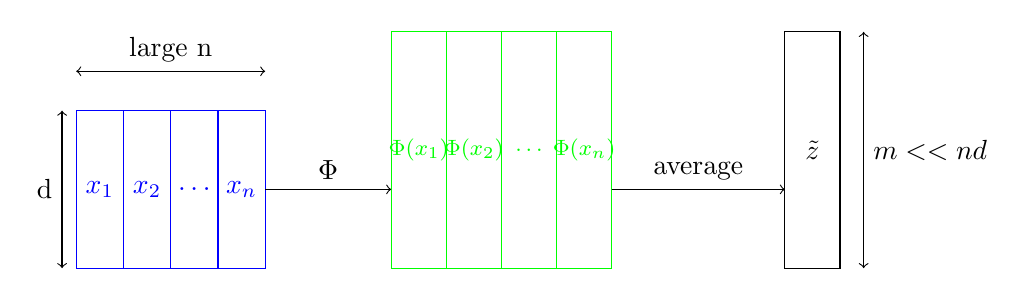
\begin{tikzpicture}
			\draw[<->] (0,2.5) -- (2.4,2.5) node[midway, above] {large n};
			\draw[<->] (-0.18, 2) -- (-0.18, 0) node[midway, left] {d};
			\draw[blue] (0, 0) rectangle (0.6, 2) node [pos = .5] {$x_{1}$};
			\draw[blue] (0.6, 0) rectangle (1.2, 2) node [pos = .5] {$x_{2}$};
			\draw[blue] (1.2, 0) rectangle (1.8, 2) node [pos = .5] {$\ldots$};
			\draw[blue] (1.8, 0) rectangle (2.4, 2) node [pos = .5] {$x_{n}$};
			
			\draw[->] (2.4,1) -- (4,1) node[midway, above] {$\Phi$};
			
			\draw[green] (4, 0) rectangle (4.7, 3) node [pos = .5] {{\footnotesize $ \Phi(x_{1})$ }};
			\draw[green] (4.7, 0) rectangle (5.4, 3) node [pos = .5] {\footnotesize{$\Phi(x_{2})$}};
			\draw[green] (5.4, 0) rectangle (6.1, 3) node [pos = .5] {\footnotesize$\ldots$};
			\draw[green] (6.1, 0) rectangle (6.8, 3) node [pos = .5] {\footnotesize$\Phi(x_{n})$};
			
			\draw[->] (6.8,1) -- (9,1) node[midway, above] {average};
			
			\draw[black] (9, 0) rectangle (9.7, 3) node [pos = .5]{$\tilde{z}$};
			\draw[<->] (10, 0) -- (10, 3) node[midway, right] {$m << nd$};
			
		\end{tikzpicture}
	\end{frame}
	
\begin{frame}{Principal Component Analysis (PCA)}
	\begin{minipage}{0.59\textwidth}
		\begin{block}{PCA}
			The goal is to find the linear subspace $P_k$ that best fits the $d$-dimensional data $\{x_i\}_{i=1}^N$ in the LS sense, i.e., find an orthogonal family of $k$ vectors $\{u_l\}_{l=1}^k$ that maximizes
			\begin{equation*}
					\sum_{l=1}^k\sum_{i=1}^N |u_l^Tx_i|^2.
			\end{equation*}
		\end{block}
	\end{minipage}
	\begin{minipage}{0.4\textwidth}
	\includegraphics[width=\textwidth]{PCA_fig}
	\end{minipage}
	A solution is the $k$-principal eigenvectors of the empirical autocorrelation matrix
	\begin{equation*}
		\hat{R} = \frac{1}{N}\sum_{i=1}^N x_ix_i^T =: \frac{1}{N}\sum_{i=1}^N \Phi(x_i).
	\end{equation*}
	$\hat{R}$ is a \emph{sketch} of our data (of dim $d^2$).
\end{frame}


\begin{frame}
	The sketch 
	\begin{equation*}
		\hat{R} = \frac{1}{N}\sum_{i=1}^N x_ix_i^T =: \frac{1}{N}\sum_{i=1}^N \Phi(x_i) \in \mathbb{R}^{d^2}
	\end{equation*}
 	is a very compressed version of the data $\{x_i\}_{i=1}^N$, \emph{but}, it still contains the geometry of the data.
	\begin{block}{CS inspired idea}
		Take $m$ random measurements\footnote{$\mathcal{M}:\mathbb{R}^{d\times d}\to \mathbb{R}^m$ satisfying RIP on matrices of rank at most $2k$.} of each sample and use the sketch defined by $\Phi(x) = \mathcal{M}(xx^T)$. Provided $m>kd$, the principal eigenvectors can be recovered.
	\end{block}

\end{frame}


\begin{frame}{$k$-means centroids}
	\begin{block}{The problem}
		The goal is to recover $k$ centroids $\{c_l\}_{l=1}^k$ from some data $\{x_i\}_{i=1}^N$ that minimize
		\begin{equation*}
			\sum_{i=1}^N \min_l ||x_i - c_l||^2.
		\end{equation*}
	\end{block}
	For $N>>1$ traditional algorithms are not very efficient because they take the whole dataset at once...
	\newline
	\emph{But}, $N>>1$ allows to use the laws of large numbers and concentration. It is reasonable to consider that the data will accumulate on small portions of the space.

\end{frame}

\begin{frame}
	\begin{block}{The binning map}
		Assume the centroids are spaced by at least $\varepsilon$ and have a norm smaller than $r$, then cover $[-r,r]^d$ by, $B=(\frac{2r}{\varepsilon})^d$, $d$-dimensional cubes (\emph{bins}). For each bin, count the average number of points that belong to it. This defines the binning map $\hat{p}\in\mathbb{R}^B_+$.
	\end{block}
	This gives us a sketch of the data, but in a large dimensional space.\newline
	\emph{But}, if the model that generated the data is "structured", i.e., the data concentrates in a few centroids, then the problem is a \emph{sparse} problem.
	\begin{block}{CS inspired idea}
		Use a Gaussian random matrix in $\mathbb{R}^{m\times N}$ and define the sketch as $\tilde z = A\hat{p}$ and solve
		\begin{equation*}
			\tilde p = argmin_{p\in\Sigma_k^+}||\tilde z - Ap||^2 
		\end{equation*}
	\end{block}
\end{frame}

\begin{frame}{Sketching estimates the underlying data-distribution}
	We can do $k$-means clustering with $m$ measures using:
		\begin{itemize}
			\item $m\geq k\log{B}$ for Gaussian sampling
			\item $m \geq k\log(k)^3\log{B}$ for DFT of $\hat{p}$
		\end{itemize}
	What if we consider the \emph{continuous} Fourier Tranform (FT) ?
	\newline
	We only know the empirical distribution $\bar p_\mathcal{X} = \frac{1}{N}\sum_{i=1}^N \delta(x_i - x)$, so
	\begin{align*}
		FT(\bar p)(\omega) &= \int_{\mathbb{R}^d} \bar p_\mathcal{X}(x) e^{-i2\pi\langle w, x\rangle}dx = \frac{1}{N}\sum_{i=1}^N e^{-i2\pi\langle w,x_i\rangle} =: \bar \Psi_{\bar p_\mathcal{X}}(\omega) \\
				&\longrightarrow^{\mathbb{E}} \bar \Psi_{p^*}(\omega) \quad\text{The "true" characteristic function at $\omega$}.
	\end{align*}
	\begin{block}{CS inspired idea}
		If the true distribution $p^*$ is "simple", then interpolating the characteristic function, using simple models, on "few" of its samples should give the true distribution.
	\end{block}
\end{frame}



\begin{frame}
		\frametitle{Parallel with signal processing}
		
		\begin{itemize}
			\item Recall that in signal processing our goal is to reconstruct a vector $x \in \mathbb{R}^{d}$ from $y = Ax + \epsilon$
			\item At first glance compressive learning setup is rather different as we deal with a large collection of vectors, rather than just one
			\item The analogy becomes clearer if we assume (as it is often the case in ML) that our vectors {$\{\boldsymbol{x}_{i}\}_{i = 1}^{n}$} are modeled as i.i.d. random vectors having a probability measure $\mathbb{P}$
			
			\item In this case we get
			$$
			\lim _{n \rightarrow \infty} \frac{1}{n} \sum_{i=1}^{n} \boldsymbol{\Phi}\left(\boldsymbol{x}_{i}\right) \stackrel{a.s.}{=} \mathbb{E_{\mathbb{P}}}[\boldsymbol{\Phi}(X)] = \mathbb{A}(\mathbb{P}),
			$$
			where $\mathbb{A}$ is a linear operator matching a probability measure to the expectation over this measure of the feature map $\boldsymbol{\Phi}$
		\end{itemize}
	\end{frame}
	
	\begin{frame}
		\frametitle{Parallel with signal processing}
		\begin{itemize}
			\item In this manner we can write
			$$
			\tilde{z} =  \frac{1}{n} \sum_{i=1}^{n} \boldsymbol{\Phi}(\boldsymbol{x}_{i}) \approx \mathbb{A}(\mathbb{P}) = \mathbb{A}(\mathbb{P}) + \epsilon
			$$
			\item Thus instead of considering a linear projection of a vector measured with noise ($x \rightarrow Ax + \epsilon$), in compressive learning we consider a linear projection of the underlying probability measured with noise: $\mathbb{P} \rightarrow \mathbb{A}(\mathbb{P}) + \epsilon$
			
			\item In signal processing the linear measurement matrix A can be chosen at random to ensure good reconstruction properties with high probability. By analogy, in compressive sensing $\boldsymbol{\Phi}$ is also often randomised
		\end{itemize}
	\end{frame}






\begin{frame}{Task driven distances}
\begin{block}{Task driven distance}
Given a loss function $L$ and probability distributions $p_X$ and $p_X^'$, we consider the distance 
\begin{equation*}
    \rho(p_X,p_{X}^{'} )=\sup_{\theta}|R^*(\theta|p_X)-R^*(\theta|p_{X}^{'})|  
\end{equation*}
where $R^*(\theta|p_X)=E_{X\sim p_X}(L(\theta)|X)$ is the expected risk under $p_X$.
\end{block}
\begin{itemize}
    \item The loss function $L$ is task specific
    \item Excess risk bounds $0\leq R^*(\theta^{*'}|p_X)-R^*(\theta^{*}|p_X)\leq 2\rho(p_X,p_{X}^{'}) $ where $\theta^*=argmin_{\theta} R^*(\theta|p_X)$ and $\theta^{*'}=argmin_{\theta} R^*(\theta|p_{X}^{'})$
    \item When $\hat{p}_X$ is the empirical distribution on the data, and $p_X$ is the true distribution, under certian conditions $\rho(\hat{p}_X,p_X)=O(\frac{1}{\sqrt{n}})$
\end{itemize}

\end{frame}

\begin{frame}{LRIP and Excess risk control}
In the compressive learning framework we are interested in an upper bound of the excess risk which is controlled by the task driven distance.
\begin{block}{
The Lower Restricted Isometry Property (LRIP) } The operator $\mathcal{A}$ is said to have the LRIP with constant $C_0$ and with respect to a parametric subfamily $\Sigma_{\theta}=\{p_{\theta}|\theta\in\Theta\}$ if
\begin{equation*}
    \rho(p_{\theta},p_{\theta^{'}})\leq C_0 ||\mathcal{A}(p_{\theta})-\mathcal{A}(p_{\theta^{'}})||
\end{equation*}
for all $p_{\theta},p_{\theta^{'}}\in\Sigma_{\theta}$
\end{block}

Excess risk bound under LRIP: for all $\theta^{'}\in\Sigma_{\theta}$ 
    \begin{equation*}
    \begin{split}
        &R^*(\tilde{\theta}|p_X)-R^*(\theta^{'}|p_X)\leq 4C_0||\mathcal{A}(p_X)-\tilde{z}||\\
        &+4C_0||\mathcal{A}(p_{\theta^{'}})-\mathcal{A}(p_X)||+2\rho(p_{\theta^{'}},p_X)
    \end{split}
    \end{equation*}

\begin{itemize}
    \item Choosing $\theta^{'}=\theta^*$, this result is interpretable in terms of modeling and sampling error
\end{itemize}

    

\end{frame}

\begin{frame}{Expected and mean kernel, MMD}
\begin{itemize}
    \item Two sources of randomness: the data and the random features used for the sketch
    \item For the random feature map we have $<\frac{1}{m}\Phi(x),\frac{1}{m}\Phi(x^{'})>=\frac{1}{m}\sum_{j=1}^m e^{-j2\pi \langle w_j,x-x^{'} \rangle}$
    \item Averaging over the random features gives the \emph{expected kernel} $k(x,x^{'})=E_w(\exp(-j2\pi<w,x-x^{'}>))$
    \item We define the \emph{mean kernel} as
    $k(p,q)=E_{x\sim p, x^{'}\sim q} k(x,x^{'})$
    \item A quantity of interest is the \texit{maximum mean discrepancy}  $MMD(p,q)=\sqrt{k(p,p)-2k(p,q)+k(q,q)}$
    \item It can be shown using concentration of measure that
     $\frac{1}{\sqrt{2}}MMD(p_{\theta},p_{\theta^{'}})\leq \frac{1}{\sqrt{m}}||\mathcal{A}(p_{\theta})-\mathcal{A}(p_{\theta^{'}})||$ when $\Sigma_{\theta}$ is a finite set
     \item When $\Sigma_{\theta}$ is infinite additional assumptions are required to ensure that the LRIP property hodls
\end{itemize}

\end{frame}

\begin{frame}{Compressed clustering, fast sketching}
\begin{itemize}
    \item In practice computing the sketch using random Fourier samples might be problematic due to the difficulty in implementing accurately the complex valued function $x\rightarrow\exp(-j2\pi x)$
    \item Using the Fast Walsh-Hadamard transform it is possible to speed up the sketching process
    \item For blocks of $2^q$ by $2^q$ matrices, we make layers of alternatively sampling Radamacher diagonal layer matrices
    followed by Hadamard matrices of dimension $2^q$ by $2^q$
    \item In general, we fit several blocks of this construction vertically and padding with zeroes until we get proper dimension for $W$
\end{itemize}

\end{frame}








\end{document}